\documentclass[letterpaper,cleveref]{lipics-v2019}

\usepackage{natbib}
\usepackage{booktabs}
\usepackage{amsmath,amsthm}
\usepackage{hyperref}
\usepackage{xcolor}

\hypersetup{
colorlinks=true,       % false: boxed links; true: colored links
linkcolor=red,          % color of internal links (change box color with
%linkbordercolor)
citecolor=blue,       % color of links to bibliography
filecolor=magenta,   % color of file links
urlcolor=cyan           % color of external links
}

%% Comments
\newif\ifcomments\commentstrue

\ifcomments
\newcommand{\authornote}[3]{\textcolor{#1}{[#3 ---#2]}}
\newcommand{\todo}[1]{\textcolor{red}{[TODO: #1]}}
\else
\newcommand{\authornote}[3]{}
\newcommand{\todo}[1]{}
\fi

\newcommand{\wss}[1]{\authornote{blue}{SS}{#1}} %Spencer Smith
\newcommand{\jc}[1]{\authornote{red}{JC}{#1}} %Jacques Carette
\newcommand{\oo}[1]{\authornote{magenta}{OO}{#1}} %Olu Owojaiye
\newcommand{\pmi}[1]{\authornote{green}{PM}{#1}} %Peter Michalski
\newcommand{\ad}[1]{\authornote{brown}{AD}{#1}} %Ao Dong

\newcommand{\notdone}[1]{\textcolor{red}{#1}}
\newcommand{\done}[1]{\textcolor{black}{#1}}

%\oddsidemargin 0mm
%\evensidemargin 0mm
%\textwidth 160mm
%\textheight 200mm

\theoremstyle{definition}
\newtheorem{defn}{Definition}

\title{Methodology for Assessing the State of the Practice for Domain X} 
\author{Spencer Smith}{McMaster University, Canada}{smiths@mcmaster.ca}{}{}
\author{Jacques Carette}{McMaster University, Canada}{carette@mcmaster.ca}{}{}
\author{Olu Owojaiye}{McMaster University, Canada}{owojaiyo@mcmaster.ca}{}{}
\author{Peter Michalski}{McMaster University, Canada}{michap@mcmaster.ca}{}{}
\author{Ao Dong}{McMaster University, Canada}{donga9@mcmaster.ca}{}{}

\authorrunning{Smith et al.}  \Copyright{Spencer Smith and Jacques Carette and
Olu Owojaiye and Peter Michalski and Ao Dong}

\date{\today}

\hideLIPIcs
\nolinenumbers

\begin{document}
\maketitle

\begin{abstract}
	...
\end{abstract}

\tableofcontents

\section{Introduction} \label{SecIntroduction}

Purpose and scope of the document.  \wss{Needs to be filled in.  Should
  reference the overall research proposal, and the ``state of the practice''
  exercise in particular.  Reference questions we are trying to answer.}

Note the following formatting conventions of this document. Red text denotes a
link to information within the document. Purple text denotes a link to
supplementary information that is external to this document. Blue text denotes a
URL link.\pmi{needs to be added to intro to explain convention}

\section{Research Questions}\label{ResearchQuestions}

The following are research questions that we want to answer in order to assess the state of practice of research software in our chosen domain:

\begin{enumerate}
\item What artifacts do current software packages produce? 
\item What tools are used by current software packages?
\item What principles, processes, and methodologies are used in the development of current software packages?
\item What are the pain points for developers working on SCS projects? What aspects of the existing processes, methodologies and tools do they consider could potentially be improved? What processes, methodologies and tools have they changed in order to reduce obstacles?
\item What are the attitudes and actions of research software developers toward:
\begin{enumerate}
\item sustainability?
\item usability?
\item modifiability?
\end{enumerate} 
\item For a given domain of research software, what current projects provide the best examples of high quality software and documentation?
\end{enumerate}

%In general questions:
%
%\begin{enumerate}
%\item Comparison between domains
%\item How to measure qualities
%\item How does the quality compare for projects with the most resources to %those
%  with the fewest?
%\item What skills/knowledge are needed by future developers?
%\item How can the development process be improved?
%\item What are the common pain points?
%\end{enumerate}
%
%For each domain questions:
%
%\begin{enumerate}
%\item Best examples within the domain
%\item What software artifacts?
%\item What are the pain points?
%\item Any advice on what can be done about the pain points?
%\end{enumerate}
%
%Measure the effort invested and the reward.  Related to sustainability.
%
%Collect the data and see what conclusions follow.  For an individual domain,
%between domains.  The process isn't so much about ranking the software as it is
%about looking at the software closely and see what conclusions arise.  The
%measurements are intended to force scrutiny, from different perspectives.

\section{Overview of Steps in Assessing Quality of the Domain Software}\label{StepsAQDS}

\begin{enumerate}
\item Start with the state of practice research questions. (Section~\ref{ResearchQuestions}) \pmi{To be updated based on feedback}
\item Identify the domain. (Section~\ref{SecIdentifyDomain}) \pmi{In second review}
\item \emph{Domain Experts}: Create a top ten list of software packages in the domain. (\href{https://github.com/smiths/AIMSS/blob/master/StateOfPractice/Methodology/Meeting Agenda withmDomainmExperts.pdf}{Meeting Agenda with Domain Experts})
\item Brief the Domain Experts on the overall objective, research proposal, research questions, measurement template, survey for short list projects, usability tests, performance benchmarks, maintainability experiments. (\href{https://github.com/smiths/AIMSS/blob/master/StateOfPractice/Methodology/Meeting Agenda withmDomainmExperts.pdf}{Meeting Agenda with Domain Experts})
\item Identify broad list of candidate software packages in the domain. (Section~\ref{SecIdentifyCandSoft})
\item Preliminary filter of software packages list. (Section~\ref{SecInitialFilter}) \pmi{To be edited based on feedback}
\item \emph{Domain Experts}: Review domain software list. (\href{https://github.com/smiths/AIMSS/blob/master/StateOfPractice/Methodology/Meeting Agenda withmDomainmExperts.pdf}{Meeting Agenda with Domain Experts})
\item Domain Analysis. (Section~\ref{SecDomainAnalysis})\pmi{To be edited - add intro}
\item \emph{Domain Experts}: Vet domain analysis. (\href{https://github.com/smiths/AIMSS/blob/master/StateOfPractice/Methodology/Meeting Agenda withmDomainmExperts.pdf}{Meeting Agenda with Domain Experts}) 
\item Gather source code and documentation for each prospective software package.
\item Collect empirical measures. (Section~\ref{SecEmpiricalMeasures})
\item Measure using measurement template. (Section~\ref{SecShallowMeasure}) \pmi{To be edited based on feedback}
\item Use AHP process to rank the software packages. (Section~\ref{SecAHP})
\item Identify a short list of top software packages, typically four to six, for deeper exploration according to the AHP rankings of the measurements.
\item \emph{Domain Experts}: Vet AHP ranking and short list. (\href{https://github.com/smiths/AIMSS/blob/master/StateOfPractice/Methodology/Meeting Agenda withmDomainmExperts.pdf}{Meeting Agenda with Domain Experts})
\item With short list:
\begin{enumerate}
\item Survey developers (\href{https://github.com/smiths/AIMSS/blob/master/StateOfPractice/Methodology/Questions to Developers.pdf}{Questions to Developers})
\item Usability experiments (\href{https://github.com/smiths/AIMSS/blob/master/StateOfPractice/Methodology/User Experiments.pdf}{User Experiments})
\item Performance benchmarks\pmi{note: this is still in consideration}
\item Maintainability experiments\pmi{note: these experiments need to be completed - to be discussed at next meeting}
\end{enumerate}
\item Rank short list. (Section~\ref{SecRankShortList}) \pmi{To be completed}
\item Document answers for research questions.
\end{enumerate}

\wss{The domain expert is involved in multiple steps in the process.  How best
  to get their feedback?  The domain experts are busy and are unlikely to devote
  significant time to the project.  We need to quickly get to the point.  Maybe
  something around task based inspection?  Directed interview?}


\section{How to Identify the Domain} \label{SecIdentifyDomain}
A domain of research software must be identified. Research software is defined in this exercise as ``software that is used to generate, process or analyze results that [are intended] to appear in a publication'' \citep{hettrick2014uk}. The chosen domain must have the following properties:

\begin{enumerate}	
	\item The domain must fall within the research software scope.
	\item The domain must be well understood.
	\item There must be a community of people studying the domain.
	\item A preliminary search, or discussion with experts, suggests that there will be numerous, at least about 15, candidate software packages to study.
	\item The software packages must have open source options. 
\end{enumerate}

Some examples of domains that fit these criteria are seismology software, as well as mesh generators and processors. These are described in \citep{SmithEtAl2018} and \citep{smith2016state}, respectively.


\section{How to Identify Candidate Software} \label{SecIdentifyCandSoft}
The candidate software can be found through search engine queries targeting authoritative lists of software from the domain, such as lists on GitHub and swMATH, and by searching domain related publications. Domain experts are also asked for their suggestions and are asked to review the list. The candidate software should have the following properties:

\begin{enumerate}
	\item Major function(s) must fall within the identified domain.
	\item Must have viewable source code.
	\item Ideally have a git repository or ability to gather empirical measures found in Section \ref{SecEmpiricalMeasures}.
	\item The software cannot be marked as incomplete or in an initial development phase.
\end{enumerate}

\section{How to Initially Filter the Software List} \label{SecInitialFilter}
The initial list of candidate software packages should first be filtered to a manageable size. Our target is about 30 packages. We want the list to include packages that are not marked as incomplete and are at least somewhat organized and understandable. We also want the list to be a good representation of the software domain, with packages having enough in common with respect to functionality that it makes sense to compare the software. The initial list of candidate software should be filtered using the following properties sequentially:

\begin{enumerate}
	\item Scope: The functionality of the domain software should be increasingly specific.
	\item Usage: The installation procedure should appear to be clear or easy to figure out.
    \item Age: Ideally the latest release or source code commit should be relatively recent, such as within the last 5 years, unless the candidate software appears to be well recommended and currently in use.
\end{enumerate}

Copies of both the initial and filtered lists should be kept for traceability purposes.

\section{Domain Analysis} \label{SecDomainAnalysis}

The domain analysis consists of a commonality analysis of the family of software packages. Its purpose is to show the relationships between these packages, and to facilitate an understanding of the informal specification and development of them. \cite{weiss1997defining} defines commonality analysis as an approach to defining a family by identifying commonalities, variabilities, and common terminology for the family. Commonalities are goals, theories, models, definitions and assumptions that are common between family members. Likewise, variabilities are goals, theories, models, definitions and assumptions that are different between family members. The final result of the domain analysis will be tables of commonalities, variabilities, and parameters of variation of a program family, which \cite{parnas1976design} defines as ``a set of programs whose common properties are so extensive that it is advantageous to study the common properties of the programs before analyzing individual members''. \cite{smith2008commonality} present a template for conducting a commonality analysis, which was referred to when conducting this work. \cite{weiss1998commonality} describes another commonality analysis technique for deciding the members of a program family which readers are encouraged to be familiar with. \cite{SmithAndChen2004} and \cite{SmithMcCutchanAndCarette2017} are examples of a commonality analysis for a family of mesh generating software and a family of material models, respectively . The steps to produce a commonality analysis are:

\begin{enumerate}
\item Write an Introduction
\item Write the Overview of Domain
\item List Commonalities
\item List Variabilities
\item List Parameters of Variation
\item Add Terminology, Definitions, Acronyms
\end{enumerate}

A sample commonality analysis for Lattice Boltzmann Solvers can be found
\href{https://github.com/smiths/AIMSS/blob/master/StateOfPractice/Peter-Notes/Commonality-Analysis-LB-Systems.pdf}{here}.

\section{Empirical Measures} \label{SecEmpiricalMeasures}
Some quality measurements rely on the gathering of raw and processed empirical data. We focus on data that is reasonably easy to collect, which we combine and analyze for this assessment. The measures that are collected relate to the research questions that we want to answer. For instance, we collect some of the data to see how large a project is. Other measures intend to ascertain a project’s popularity, or how active the project is.
Section \ref{rawdata} will orient the reader as to what raw data is collected. 
Some of this data can be observed from Git repository metrics. The rest can be collected using freeware tools. \href{https://github.com/tomgi/git_stats}{GitStats} is used to measure the number of binary files as well as the number of added and deleted lines in a repository. The tool is also used to measure the number of commits over different intervals of time. \href{https://github.com/boyter/scc}{Sloc Cloc and Code (scc)} is used to measure the number of text based files as well as the number of total, code, comment, and blank lines in a repository. These tools were selected due to their installability, usability, and ability to gather the empirical measures listed below. A guide for installing and running them can be found \href{https://github.com/smiths/AIMSS/blob/master/StateOfPractice/Methodology/A Guide to Empirical Measures.pdf}{here}. Section \ref{processeddata} introduces the required processed data, which is calculated using the raw data.

\subsection{Raw Data}\label{rawdata}
The following raw data measures are extracted from repositories:

\begin{itemize}
\item Number of stars.
\item Number of forks.
\item Number of people watching the repository.
\item Number of open pull requests.
\item Number of closed pull requests.	
\item Number of developers.	
\item Number of open issues.
\item Number of closed issues.
\item Initial release date.
\item Last commit date.
\item Programming languages used.
\item Number of text-based files.
\item Number of total lines in text-based files.
\item Number of code lines in text-based files.
\item Number of comment lines in text-based files.
\item Number of blank lines in text-based files.
\item Number of binary files.  
\item Number of total lines added to text-based files.
\item Number of total lines deleted from text-based files.
\item Number of total commits.
\item Numbers of commits by year in the last 5 years. (Count from as early as possible if the project is younger than 5 years.) 
\item Numbers of commits by month in the last 12 months.
\end{itemize}


\subsection{Processed Data}\label{processeddata}
The following measures are calculated from the raw data:

\begin{itemize}
\item Status of software package (dead or alive). Alive is defined as the presence of repository commits or software package version releases in the last 18 months.
\item Percentage of identified issues that are closed.
\item Percentage of code that is comments.
\end{itemize}

\section{Measure Using Measurement Template} \label{SecShallowMeasure}

\begin{figure}[h!]
	\begin{center}
		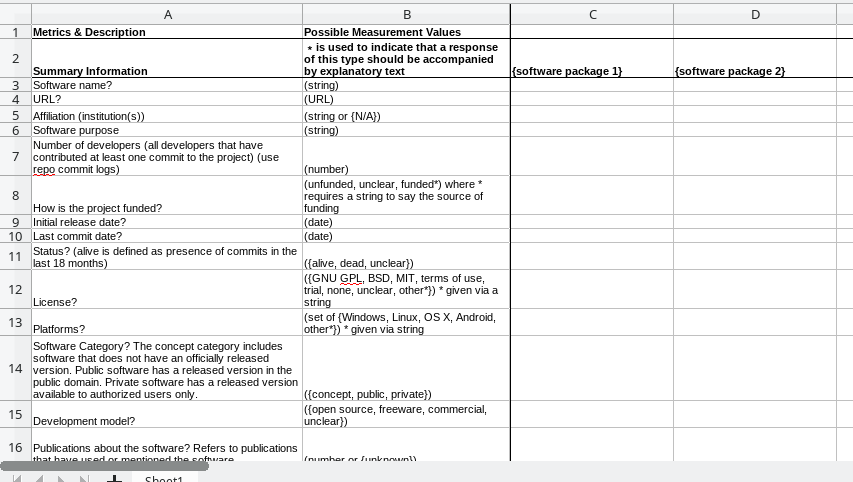
\includegraphics[width=1.0\textwidth]{measurement_template}
		\caption{Top of Measurement Template}
		\label{measurement_template_image}

	\end{center}
\end{figure}

The \href{https://github.com/smiths/AIMSS/blob/master/StateOfPractice/Methodology/Combined_MeasurementTemplate_EmpiricalMeasures.xlsx}{Measurement Template} is used to track measurements and quality scores for all of the software packages in the domain. For each software package, fill out one column of the template. This process can take between 2 to 5 hours for each package.
Project developers can be contacted for help regarding installation, if necessary, but a cap of about 2 hours should be imposed on the entire installation process. For completing the template, please follow these steps:

\pmi{SS:"explain any tricky parts with interpreting the parameters of variation for measuring a particular indicator. A few example would help."}\pmi{Ask Ao for input}

\begin{enumerate} 
	\item Gather the summary information into the top section of the document (Figure \ref{measurement_template_image})
	\item Using the GitStats tool that is described in Section \ref{SecEmpiricalMeasures} gather the measurements for the Repo Metrics - GitStats section found near the bottom of the document
	\item Using the SCC tool that is also described in Section \ref{SecEmpiricalMeasures} gather the measurements for the Repo Metrics - SCC section found near the bottom of the document
	\item If the software package is found on git, gather the measurements for the Repo Metrics - GitHub section found near the bottom of the document
	\item Review installation documentation and attempt to install the software package on a virtual machine
	\item Gather the measurements for installability
	\item Gather the measurements for correctness and verifiability
	\item Gather the measurements for surface reliability
	\item Gather the measurements for surface robustness
	\item Gather the measurements for surface usability
	\item Gather the measurements for maintainability
	\item Gather the measurements for reusability
	\item Gather the measurements for surface understandability
	\item Gather the measurements for visibility and transparency
	\item Assign a score out of ten for each quality. The score can be measured using the \href{https://github.com/smiths/AIMSS/blob/master/StateOfPractice/Methodology/MeasurementTemplate_ImpressionCalculator.xlsx}{Measurement Template Impression Calculator}. For each quality measurement, the file indicates the appropriate score to assign the measurement based on possible measurement values.
\end{enumerate}

\section{Analytic Hierarchy Process} \label{SecAHP}
The Analytical Hierarchy Process (AHP) is a decision-making technique that can be used when comparing multiple options by multiple criteria. In our work AHP is used for comparing and ranking the software packages of a domain using the quality scores that are gathered in the \href{https://github.com/smiths/AIMSS/blob/master/StateOfPractice/Methodology/Combined_MeasurementTemplate_EmpiricalMeasures.xlsx}{Measurement Template}. AHP performs a pairwise analysis between each of the quality options using a matrix which is then used to generate an overall score for each software package for the given criteria. \cite{SmithEtAl2016} shows how AHP is applied to ranking software based on quality measures. We have developed a tool for conducting this process. The tool includes an AHP JAR script and a sensitivity analysis JAR script that is used to ensure that the software package rankings are appropriate with respect to the uncertainty of the quality scores. The README file of the tool is found \href{https://github.com/smiths/AIMSS/blob/master/StateOfPractice/AHP2020/LBM/README.txt}{here}. This file outlines the requirements for, and configuration and usage of, the JAR scripts. The JAR scripts, source code, and required libraries are located in the same folder as the README file.

\section{Rank Short List} \label{SecRankShortList}
Rank using pairwise comparison of short list software packages with respect to usability survey results.

\pmi{SS: let's ask the people that do the usability/performance/maintainability experiments to do an AHP pair-wise comparison between the short-list software packages}

\section{Quality Specific Measures}

\subsection{\notdone{Installability} \oo{owner}}

\subsection{\notdone{Correctness} \oo{owner}}

\subsection{\notdone{Verifiability/Testability} \oo{owner}}

\subsection{\notdone{Validatability} \oo{owner}}

\subsection{\notdone{Reliability} \oo{owner}}

\subsection{\notdone{Robustness} \pmi{owner}}

\subsection{\notdone{Performance} \pmi{owner}}

\subsection{\notdone{Usability} \jc{owner}} 

\subsection{\notdone{Maintainability} \pmi{owner}}

\subsection{\notdone{Reusability} \pmi{owner}}

\subsection{\notdone{Portability} \pmi{owner}}

\subsection{\notdone{Understandability} \jc{owner}}

\subsection{\notdone{Interoperability} \ad{owner}}

\subsection{\notdone{Visibility/Transparency} \ad{owner}}

\subsection{\notdone{Reproducibility} \wss{owner}}

\subsection{\notdone{Productivity} \ad{owner}}

\subsection{\notdone{Sustainability} \wss{owner}}

\subsection{\notdone{Completeness} \ad{owner}}

\subsection{\notdone{Consistency} \ad{owner}}

\subsection{\notdone{Modifiability} \jc{owner}}

\subsection{\notdone{Traceability} \jc{owner}}

\subsection{\notdone{Unambiguity} \wss{owner}}

\subsection{\notdone{Verifiability} \wss{owner}}

\subsection{\notdone{Abstract} \wss{owner}}

\section{Using Data to Rank Family Members}

Describe AHP process (or similar).

\appendix
\section{Appendix}
\subsection{Survey for the Selected Projects}
\ad{Several questions are borrowed from \href{https://gitlab.cas.mcmaster.ca/smiths/pub/-/blob/master/Jegatheesan2016.pdf}{Jegatheesan2016}, and needed to be cited later.}
\subsubsection{Information about the developers and users}
\begin{enumerate}
\item Interviewees' current position/title? degrees?
\item Interviewees' contribution to/relationship with the software?
\item Length of time the interviewee has been involved with this software?
\item How large is the development group?
\item What is the typical background of a developer?
\item How large is the user group?
\item What is the typical background of a user?
\end{enumerate}

\subsubsection{Information about the software}

\begin{enumerate}
\item \ad{General} What is the most important software quality(ies) to your work? (set of selected qualities plus "else")
\item \ad{General} Are there any examples where the documentation helped? If yes, how it helped. ({yes$^*$, no})
\item \ad{General} Is there any documentation you feel you should produce and do not? If yes, what is it and why? ({yes$^*$, no})
\item \ad{Completeness} Do you address any of your quality concerns using documentation? If yes, what are the qualities and the documents. ({yes$^*$, no})
\item \ad{Visibility/Transparency} Is there a certain type of development methodologies used during the development? (\{Waterfall, Scrum, Kanban, else\})
\item \ad{Visibility/Transparency} Is there a clearly defined development process? If yes, what is it. (\{yes$^*$, no\})
\item \ad{Visibility/Transparency} Are there any project management tools used during the development? If yes, what are they. (\{yes$^*$, no\})
\item \ad{Visibility/Transparency} Going forward, will your approach to documentation of requirements and design
change? If not, why not. (\{yes, no$^*$\})
\item \ad{Correctness and Verifiability} During the process of development, what tools or techniques are used to build confidence of correctness? (string)
\item \ad{Correctness and Verifiability} Do you use any tools to support testing? If yes, what are they. (e.g. unit testing tools, regression testing suites) (\{yes$^*$, no\})
\item \ad{Correctness and Verifiability} Is there any document about the requirements specifications of the program? If yes, what is it. (\{yes$^*$, no\})
\item \ad{Portability} Do you think that portability has been achieved? If yes, how? (\{yes$^*$, no\})
\item \ad{Maintainability} How was maintainability considered in the design? (string)
\item \ad{Maintainability} What is the maintenance type? (set of \{corrective, adaptive, perfective,
unclear\})
\item \ad{Reusability} How was reusability considered in the design? (string)
\item \ad{Reusability} Are any portions of the software used by another package? If yes, how they are used. ({yes$^*$, no})
\item \ad{Reproducibility} Is reproducibility important to you? ({yes$^*$, no})
\item \ad{Reproducibility} Do you use tools to help reproduce previous software results? If yes, what are they. (e.g. version control, configuration management) ({yes$^*$, no})
\item \ad{Completeness} Is any of the following documents used during the development? ({yes$^*$, no})
\item \ad{General} Will this experience influence how you develop software? Do you see yourself maintaining the same level of documentation, tool support as you go forward? (string)
\begin{itemize}
\item Module Guide
\item Module Interface Specification
\item Verification and Validation Plan
\item Verification and Validation Report
\end{itemize}
\end{enumerate}

\subsection{Empirical Measures Considerations - Raw Data}

Measures that can be extracted from on-line repos.

\ad{Still at brainstorm stage.}
\begin{itemize}
	\item number of contributors
	\item number of watches
	\item number of stars
	\item number of forks
	\item number of clones
	\item number of commits
	\item number of total/code/document files
	\item lines of total/logical/comment code
	\item lines/pages of documents (can pdf be extracted?)
	\item number of total/open/closed/merged pull requests
	\item number of total/open/closed issues
	\item number of total/open/closed issues with assignees
\end{itemize}

Instead of only focus on the current status of the above numbers, we may find
the time history of them to be more valuable. For example, the number of
contributors over time, the number of lines of code over time, the number of
open issues over time, etc.

\subsection{Empirical Measures Considerations - Processed Data}
Metrics that can be calculated from the raw data.

\ad{Still at brainstorm stage.}
\begin{itemize}
	\item percentage of total/open/closed issues with assignees -
	Visibility/Transparency
	\item lines of new code produced per person-month - Productivity
	\item lines/pages of new documents produced per person-month - Productivity
	\item number of issues closed per person-month - Productivity
	\item percentage of comment lines in the code - maintainability \ad{Not Ao's
		qualities}
\end{itemize}

In the above calculations, a month can be determined to be 30 days.

\subsection{Empirical Measures Considerations - Tool Tests}
\ad{This section is currently a note of unorganized contents. Most parts will beremoved or relocated.}

\ad{This citation needs to be deleted later. It's here because my compiler
	doesn't work with 0 citations}
\cite{Emms2019}

Most tests were done targeting to the repo of 3D Slicer
\href{https://github.com/tomgi/git_stats}{GitHub repo}

\subsubsection{git-stats}
\href{https://github.com/tomgi/git_stats}{GitHub repo}

Test results:
\href{http://git-stats-slicer.ao9.io/}{http://git-stats-slicer.ao9.io/} the
results are output as webpages, so I hosted for you to check. Data can be
downloaded as spreadsheets.


\subsubsection{scc}
\href{https://github.com/boyter/scc}{GitHub repo}


\subsubsection{git-of-theseus}
\href{https://github.com/erikbern/git-of-theseus}{GitHub repo}

Test results: It took about 100 minutes for one repo on a 8 core 16G ram Linux
machine. It only outputs graphs.

\subsubsection{hercules}
\href{https://github.com/src-d/hercules}{GitHub repo}

Test results: this one seems to be promising, but the installation is
complicated with various errors.

\subsubsection{git-repo-analysis}
\href{https://github.com/larsxschneider/git-repo-analysis}{GitHub repo}

\subsubsection{HubListener}
\href{https://github.com/pjmc-oliveira/HubListener}{GitHub repo}

The data that HubListener can extract.

Raw:
\begin{itemize}
	\item Number of Files
	\item Number of Lines
	\item Number of Logical Lines
	\item Number of Comments
\end{itemize}

Cyclomatic:
\href{https://www.geeksforgeeks.org/cyclomatic-complexity/}{Intro}
\begin{itemize}
	\item Cyclomatic Complexity
\end{itemize}

Halstead:
\href{https://www.geeksforgeeks.org/software-engineering-halsteads-software-metrics/}{Intro}
\begin{itemize}
	\item Halstead Effort
	\item Halstead Bugs
	\item Halstead Length
	\item Halstead Difficulty
	\item Halstead Time
	\item Halstead Vocabulary
	\item Halstead Volume
\end{itemize}

Test results: HubListener works well on the repo of itself, but it did not work
well on some other repos.

\subsubsection{gitinspector}
\href{https://github.com/ejwa/gitinspector}{GitHub repo}

Test results: it doesn't work well. Instead of creating output results, it
prints the results directly in the console.





\newpage

\bibliographystyle {plainnat}
\bibliography {../../CommonFiles/ResearchProposal}

\end{document}